% Add a Section about experimental results and verification of your output. 

% Any number, both final and intermediate results should be described. Even the experimental setup, and the measurement environment should be described. The measure should be reproducible by the readers. Listing the models of the instrument is not important (e.g.,  oscilloscope TD98445.... ), while the type of instrumentation or the type of measure is fundamental to repeat the experiment. \\
% \\
% In case, please, provide a shared folder (e.g., github, gitlab, Google Drive, ... ) where the code is available for repeat the experiments, the achieved results are available for a comparison. 

% The aim of this project was to identify the parameters of the different TEC modules and define which was the optimal one for the given application.
We estimate the internal resistance and the Seeback coefficient with a MATLAB script.
\subsection{Fitting Seeback coefficient}

The \textbf{Seebeck coefficient} (also known as thermopower, thermoelectric power, and thermoelectric sensitivity) of a material is a measure of the magnitude of an induced thermoelectric voltage in response to a temperature difference across that material, as induced by the Seebeck effect \cite{seebeckCoefficientWikipedia}, which is described by the equation \ref{eq:seeback}. It is one of the components of the figure of merit, which measures the overall efficiency of a thermoelectric device.

\begin{equation}
    S = \frac{ \Delta V}{\Delta T }
    \label{eq:seeback}
\end{equation}

As described in section \ref{sec:voc-measurement}, we can assume that we are measuring directly point A in figure \ref{fig:oc_model}. In this way, the voltage measured is dependent only on the Seeback coefficient, which in itself depends on the delta temperature between hot and cold. In MATLAB the model is written as follows:

\begin{lstlisting}[
    frame=single,
    numbers=none,
    style=Matlab-editor,
    basicstyle=\tiny,
]
% Seeback inline function
% T is a vector of mean temperature between hot and cold surfaces
seeback_coeff_mdl = @(coeffs, T)(coeffs(1));
% Model of the Open Circuit Voltage
voc_mdl = @(seeback_coeffs, T)(seeback_coeff_mdl(seeback_coeffs, T(:,1)) .* T(:,2));
% Create data table
tbl = table(mean_surface_temperature, delta_surface_temperature, measured_voltage);
% Fit model with initial guesses for each coefficient
nlm = fitnlm(tbl, voc_mdl, [0.0, 0.01, 0.02, 0.01],'Options',statset('Display','final','Robust','On'));
\end{lstlisting}

\begin{figure}[h]
    \centering
    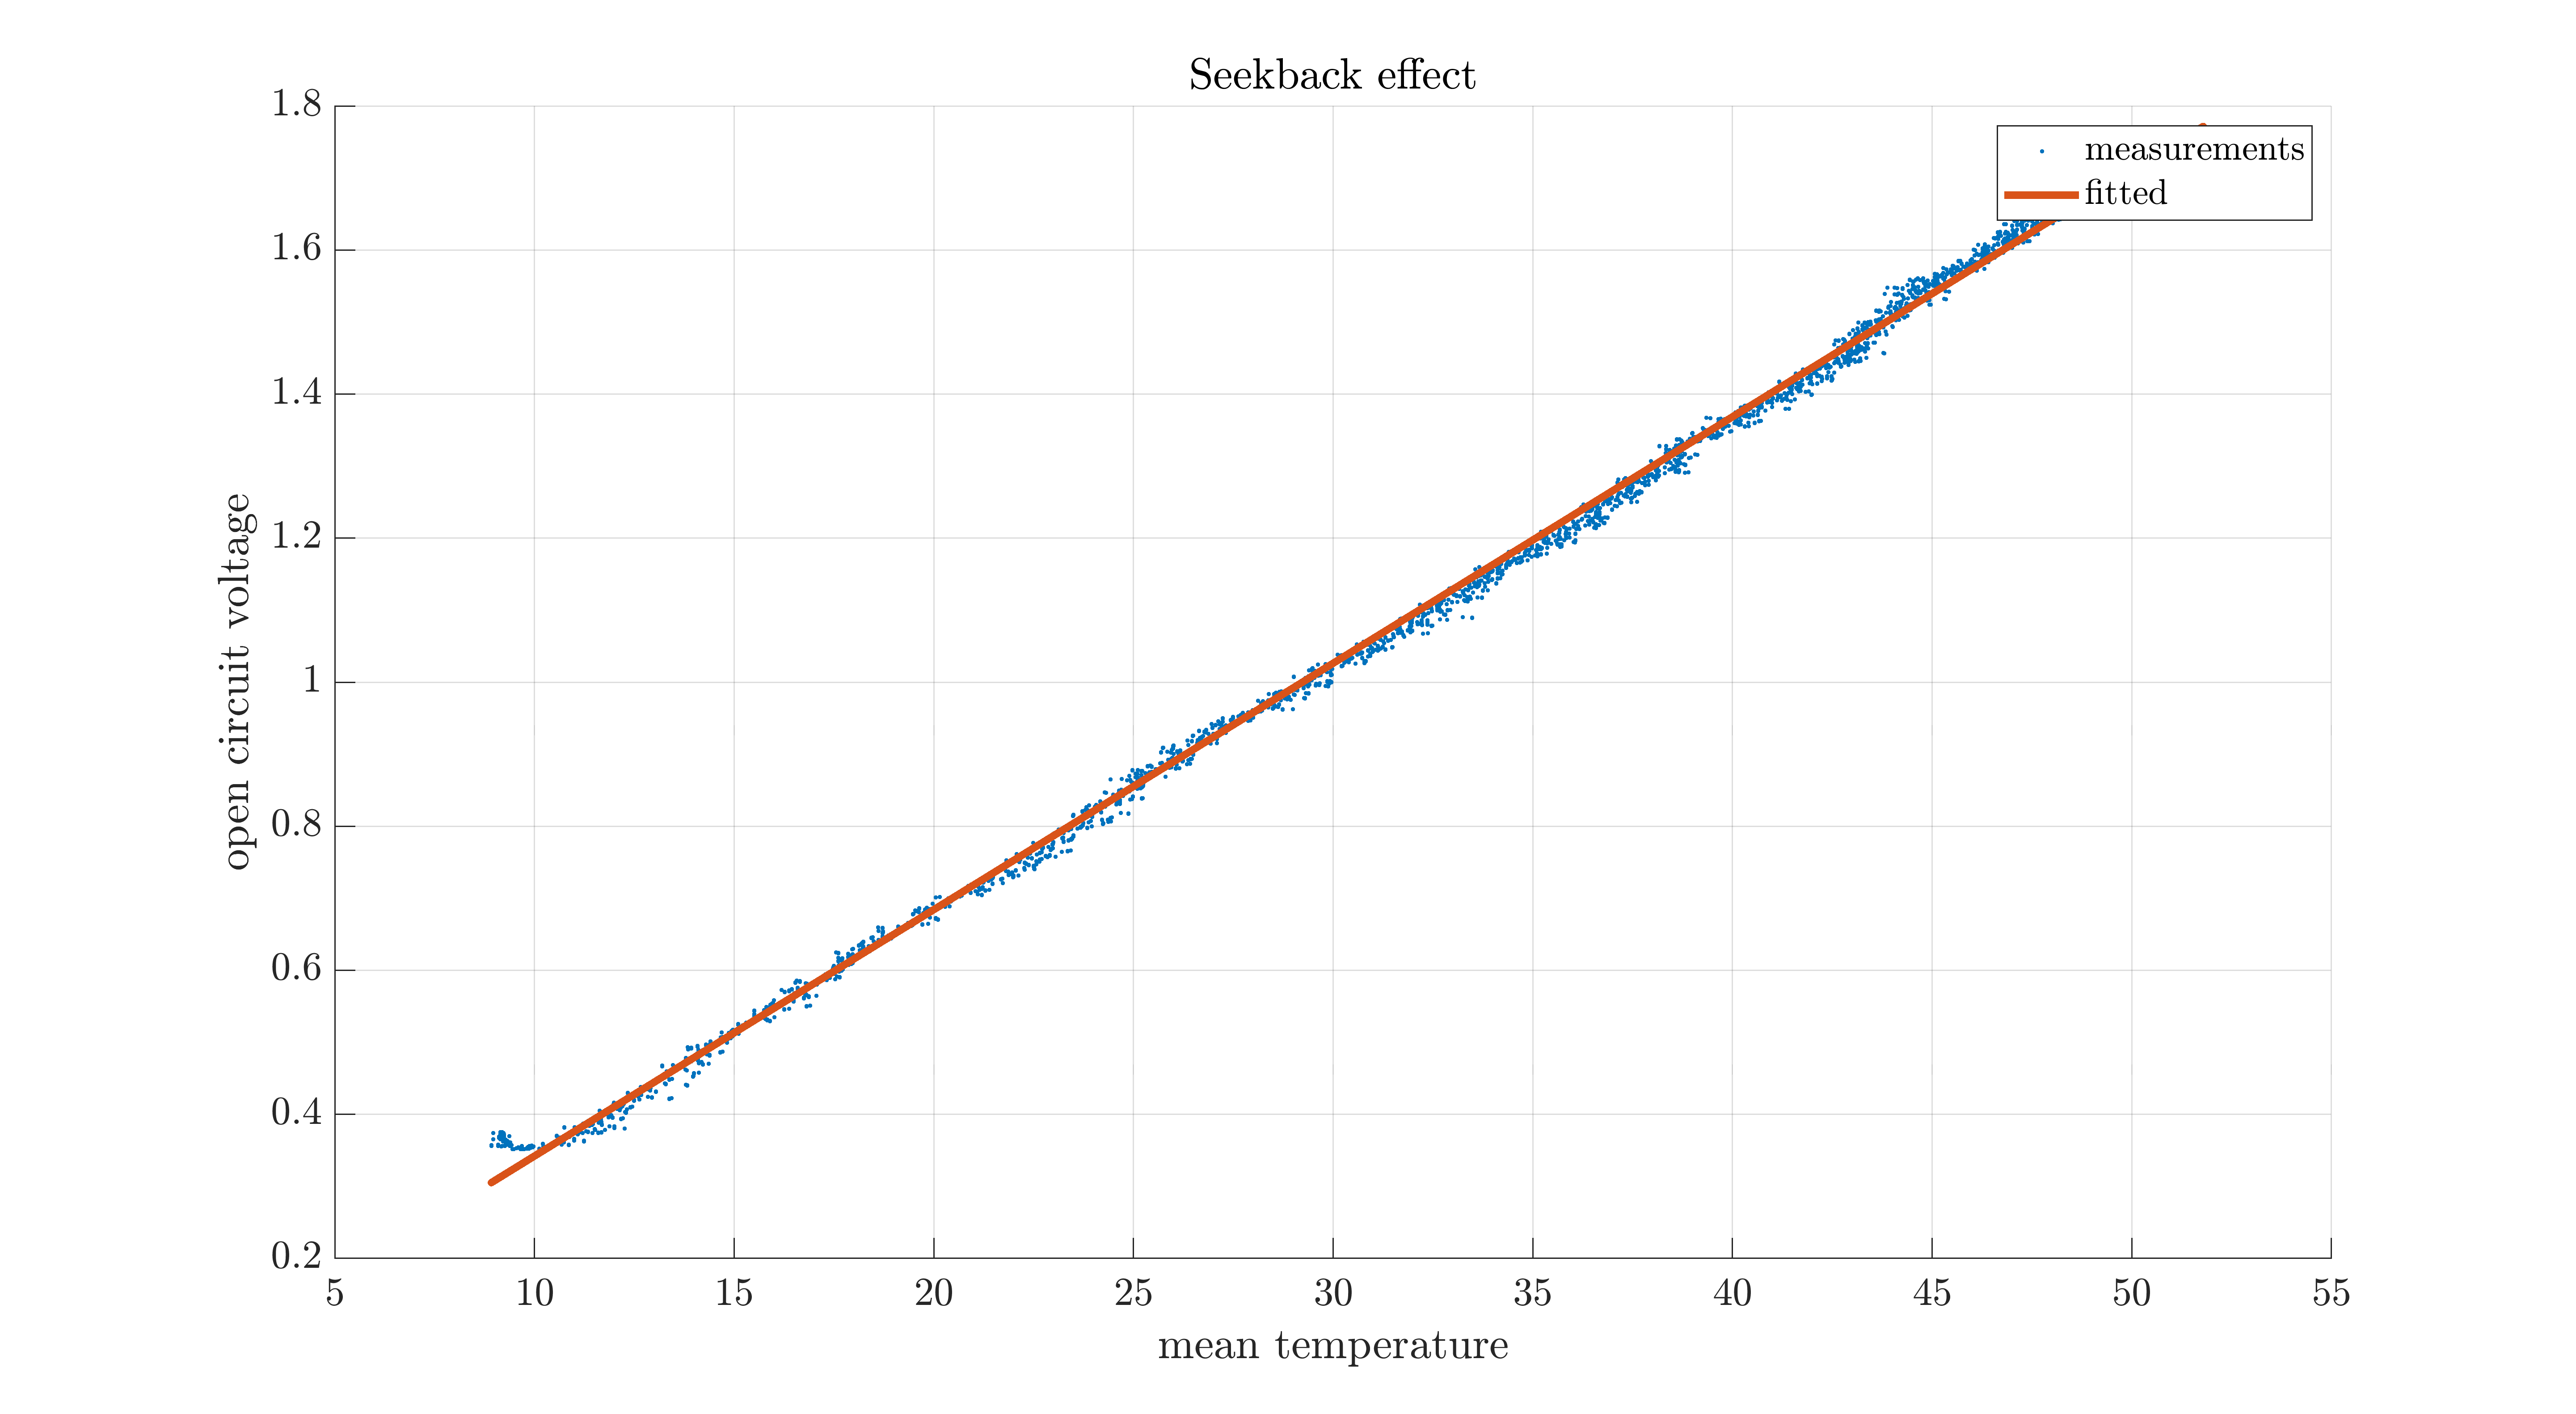
\includegraphics[width=0.45\textwidth]{assets/Seekback effect.png}
    \caption{Open circuit voltage mean temperature dependence}
    \label{fig:voc_dep_t}
\end{figure}
\begin{figure}[h]
    \centering
    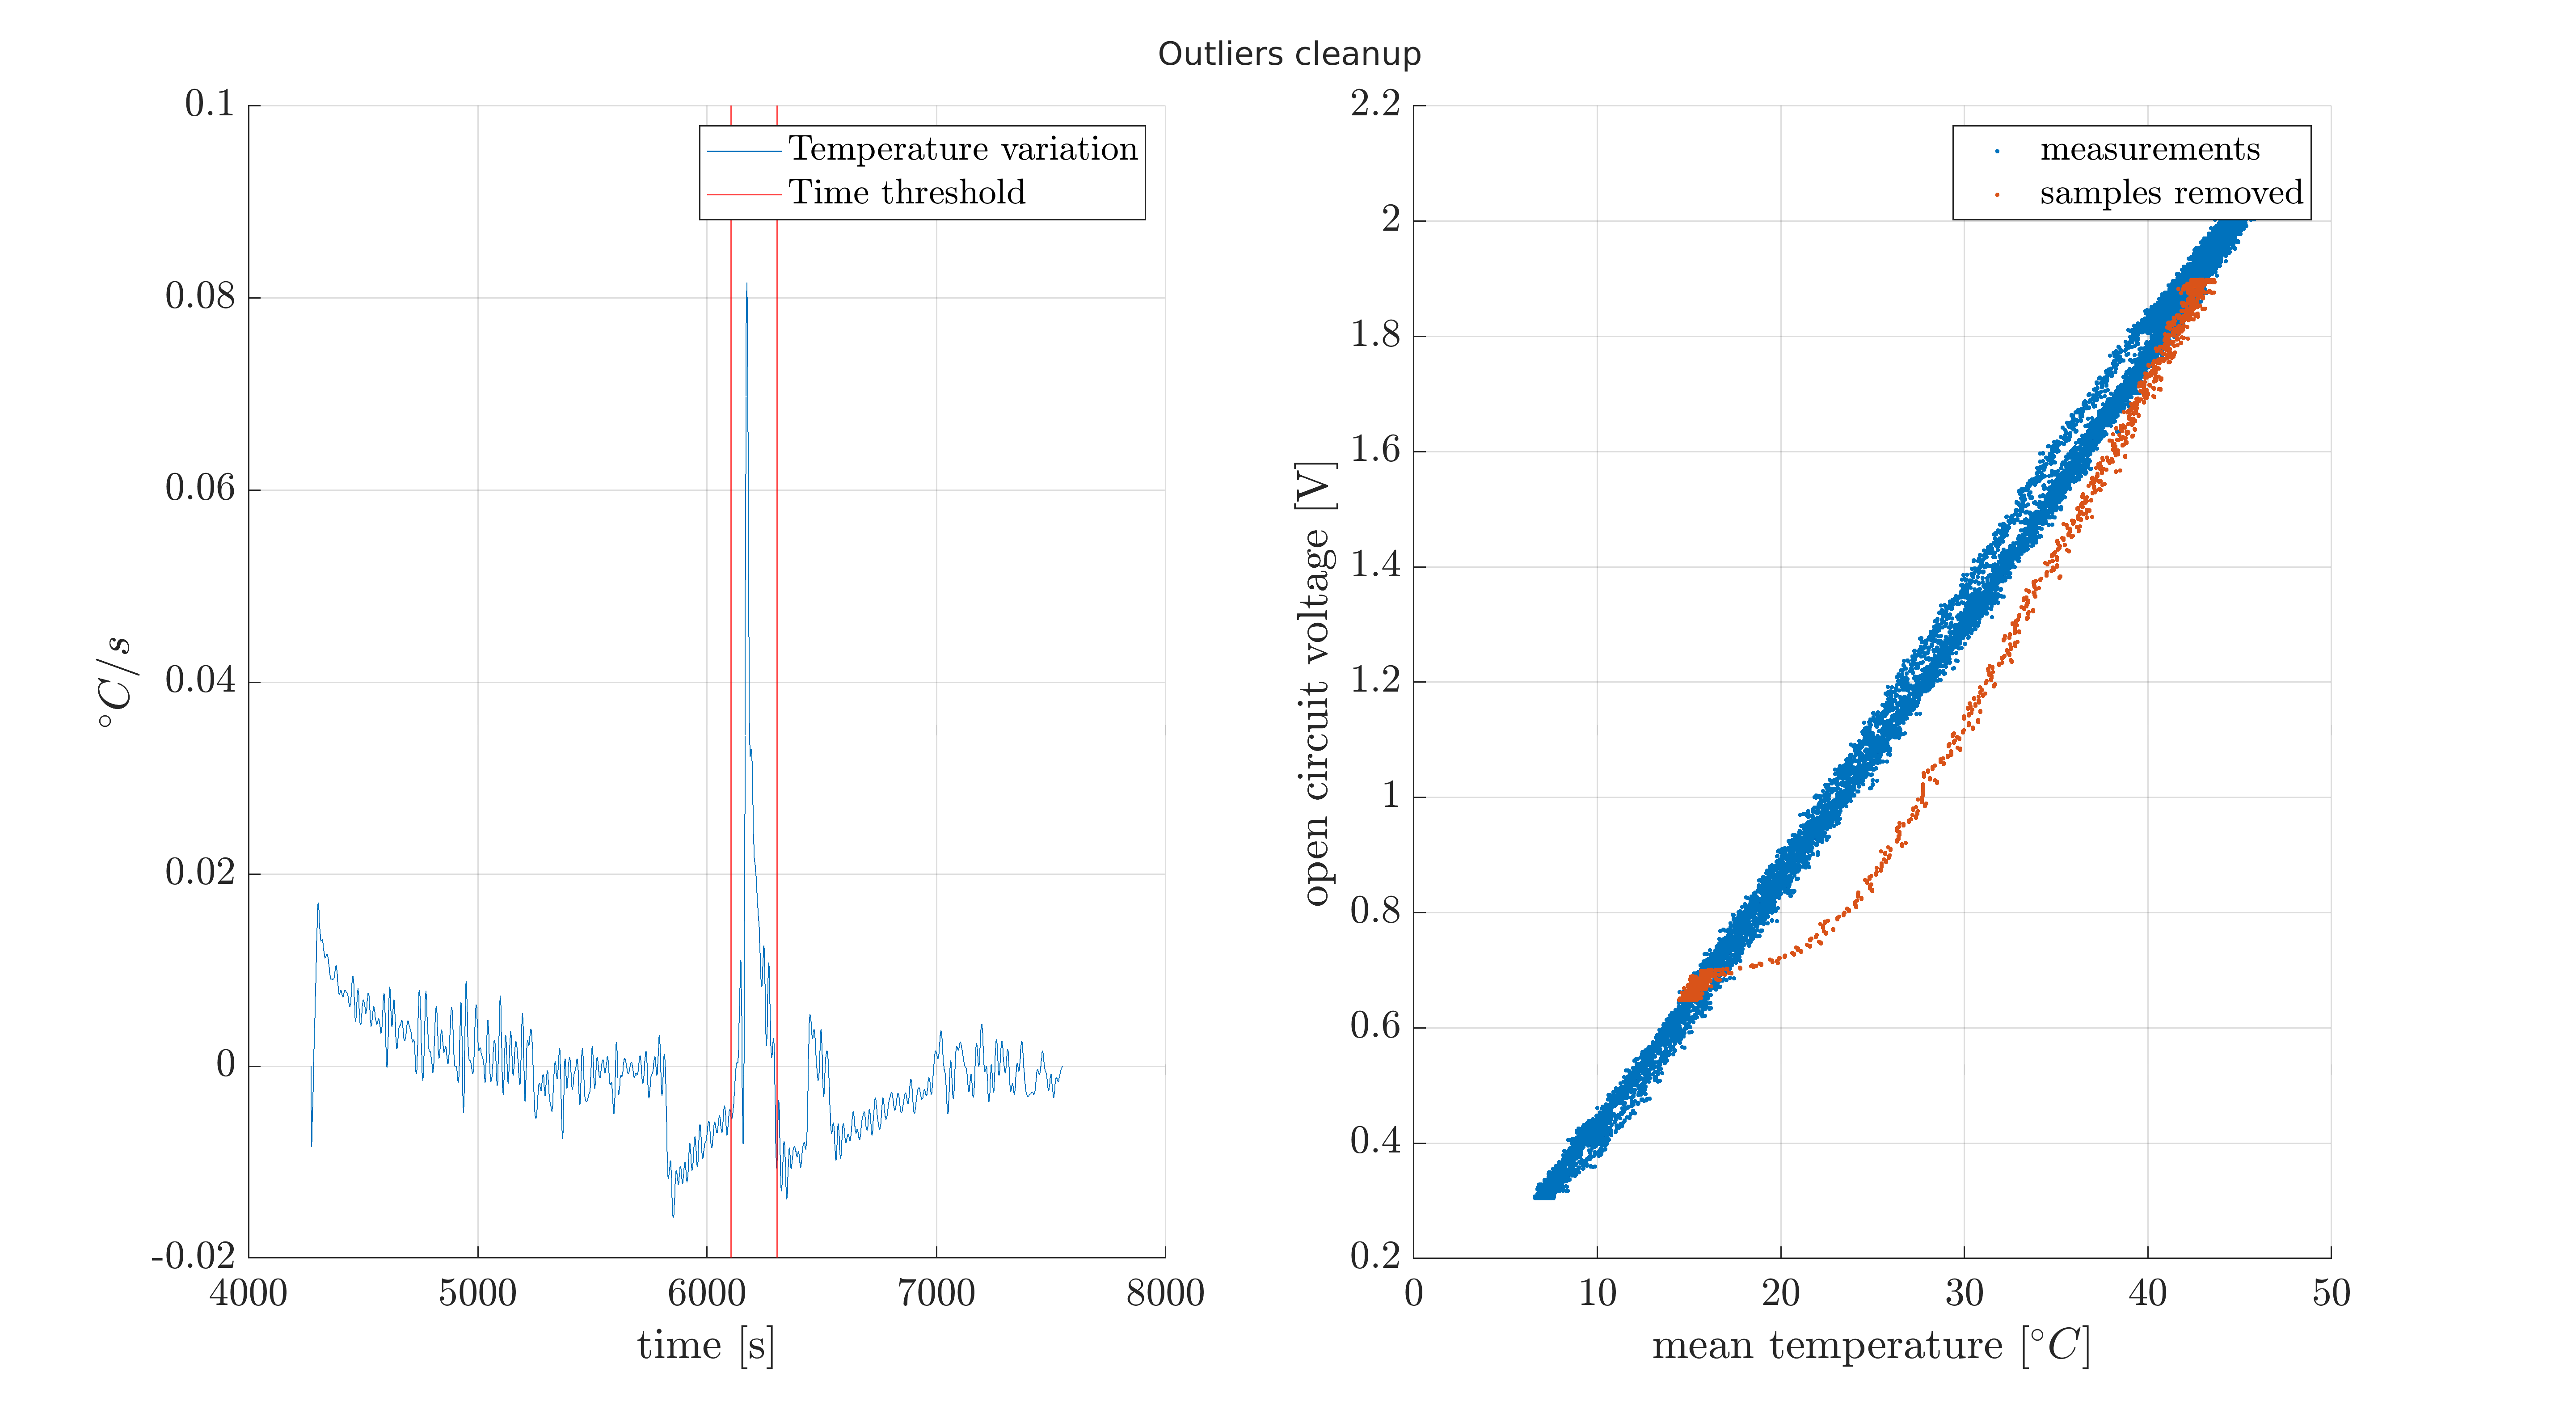
\includegraphics[width=0.45\textwidth]{assets/Outliers cleanup.png}
    \caption{Cleanup of outliers from an experiment contaimnation.}
    \label{fig:voc_cleanup}
\end{figure}

% Come raffigurato in figura\ref{fig:voc_dep_t}, dal momento che i dati non sono sovrapposti a una linea, sembrerebbe che il coefficiente di Seebeck non sia dipendente solamente dalla differenza di temperatura, ma anche dalla temperatura media. Questo tuttavia non è vero, perché il coefficiente di Seeback è di per sè una costante del materiale e dalla forma. Per questo motivo, abbiamo analizzato i dati focalizzandoci sulla variazione della temperatura media nel tempo, quindi filtrata e derivata rispetto al tempo. Il risultato mostra un picco nella variazione di temperatura, causato da qualche evento esterno che ha contaminato le letture. Abbiamo quindi tolto gli outliers e rifatto il fitting, con i risultati mostrati in figura \ref{fig:voc_cleanup}

An anomaly in the data stands out. As depicted in figure\ref{fig:voc_dep_t}, since the data are not superimposed on a line, it would appear that the Seebeck coefficient is not only dependent on the temperature difference, but also on the mean temperature. However, this is not true, because the Seeback coefficient is itself a constant of the material and from the shape. For this reason, we analyzed the data by focusing on the change in mean temperature over time, then filtered and derived with respect to time. The result shows a spike in the temperature variation, caused by some external event that contaminated the readings. We then removed the outliers and ran again the fitting, with the results shown in Figure \ref{fig:voc_cleanup}.


% Sappiamo che la scelta scientificamente più corretta sarebbe stato ripetere l'esperimento, ma raccogliere dati del tutto precisi è molto complicato, ci siamo accorti di questo problema solo in fase di analisi e togliendo lo spike di errore sono dati comunque validi.

% The Seeback coefficient is in itself a polynomial which is dependent on the mean temperature, this contribution was added after noticing that in a plot with measured voltage dependent on delta temperature, the data was not lying on a line, but seemed to have a dependency on mean temperature. Since Seeback coeeficient is a material and shape constant, it should be not dependent on mean temperature. To addess this problem we analyzed the single event that could have caused the wrong readings. In particular we focused on the variation of mean temperature in time, so we filtered the readings and differentiated it with respect to time, the result shows a spike in the temperature variation. This behaviour was caused by some external event that contaminated the readings. We then removed the outliers and the fit was done again, the result is shown in figure \ref{fig:voc_cleanup}.

\subsection{Fitting internal resistance}
We modeled the internal resistance as a constant plus a linear term dependent on the mean temperature. 
The equations used to fit the model are:
\begin{align}
    \begin{split}
    R_{int} &= R_{int_0} + R_{int_1} \cdot \overline{T} \\
    V_{OC} &= S \cdot \Delta T \\
    I &= \frac{V_{OC}}{R_{int} + R_{load}}
    \end{split}
\end{align}
The internal resistance was fitted with the following MATLAB code:

\begin{lstlisting}[
    frame=single,
    numbers=none,
    style=Matlab-editor,
    basicstyle=\tiny,
]
% Model of internal resistance
internal_resistance_mdl = @(internal_resistance_coeffs, mT_dT)(internal_resistance_coeffs(1) + internal_resistance_coeffs(2) * mT_dT(:,1));
% Model of current given a load resistance value
current_mdl = @(internal_resistance_coeffs, mT_dT_Voc)(mT_dT_Voc(:,3) ./ (load_value + internal_resistance_mdl(internal_resistance_coeffs, [mT_dT_Voc(:,1), mT_dT_Voc(:,2)])));

% Define residuals function (RMSE)
residuals = @(coeffs)(residuals_function(I, current_mdl(coeffs, [mT, dT, Voc])));

% Minimize residuals with contraints
default_options = optimoptions('fmincon');
fitted_internal_resistance_coeffs = fmincon(residuals, [0.5, 0],[],[],[],[], [0, 0], [5, inf], [], default_options);
\end{lstlisting}

\begin{figure}[h]
    \centering
    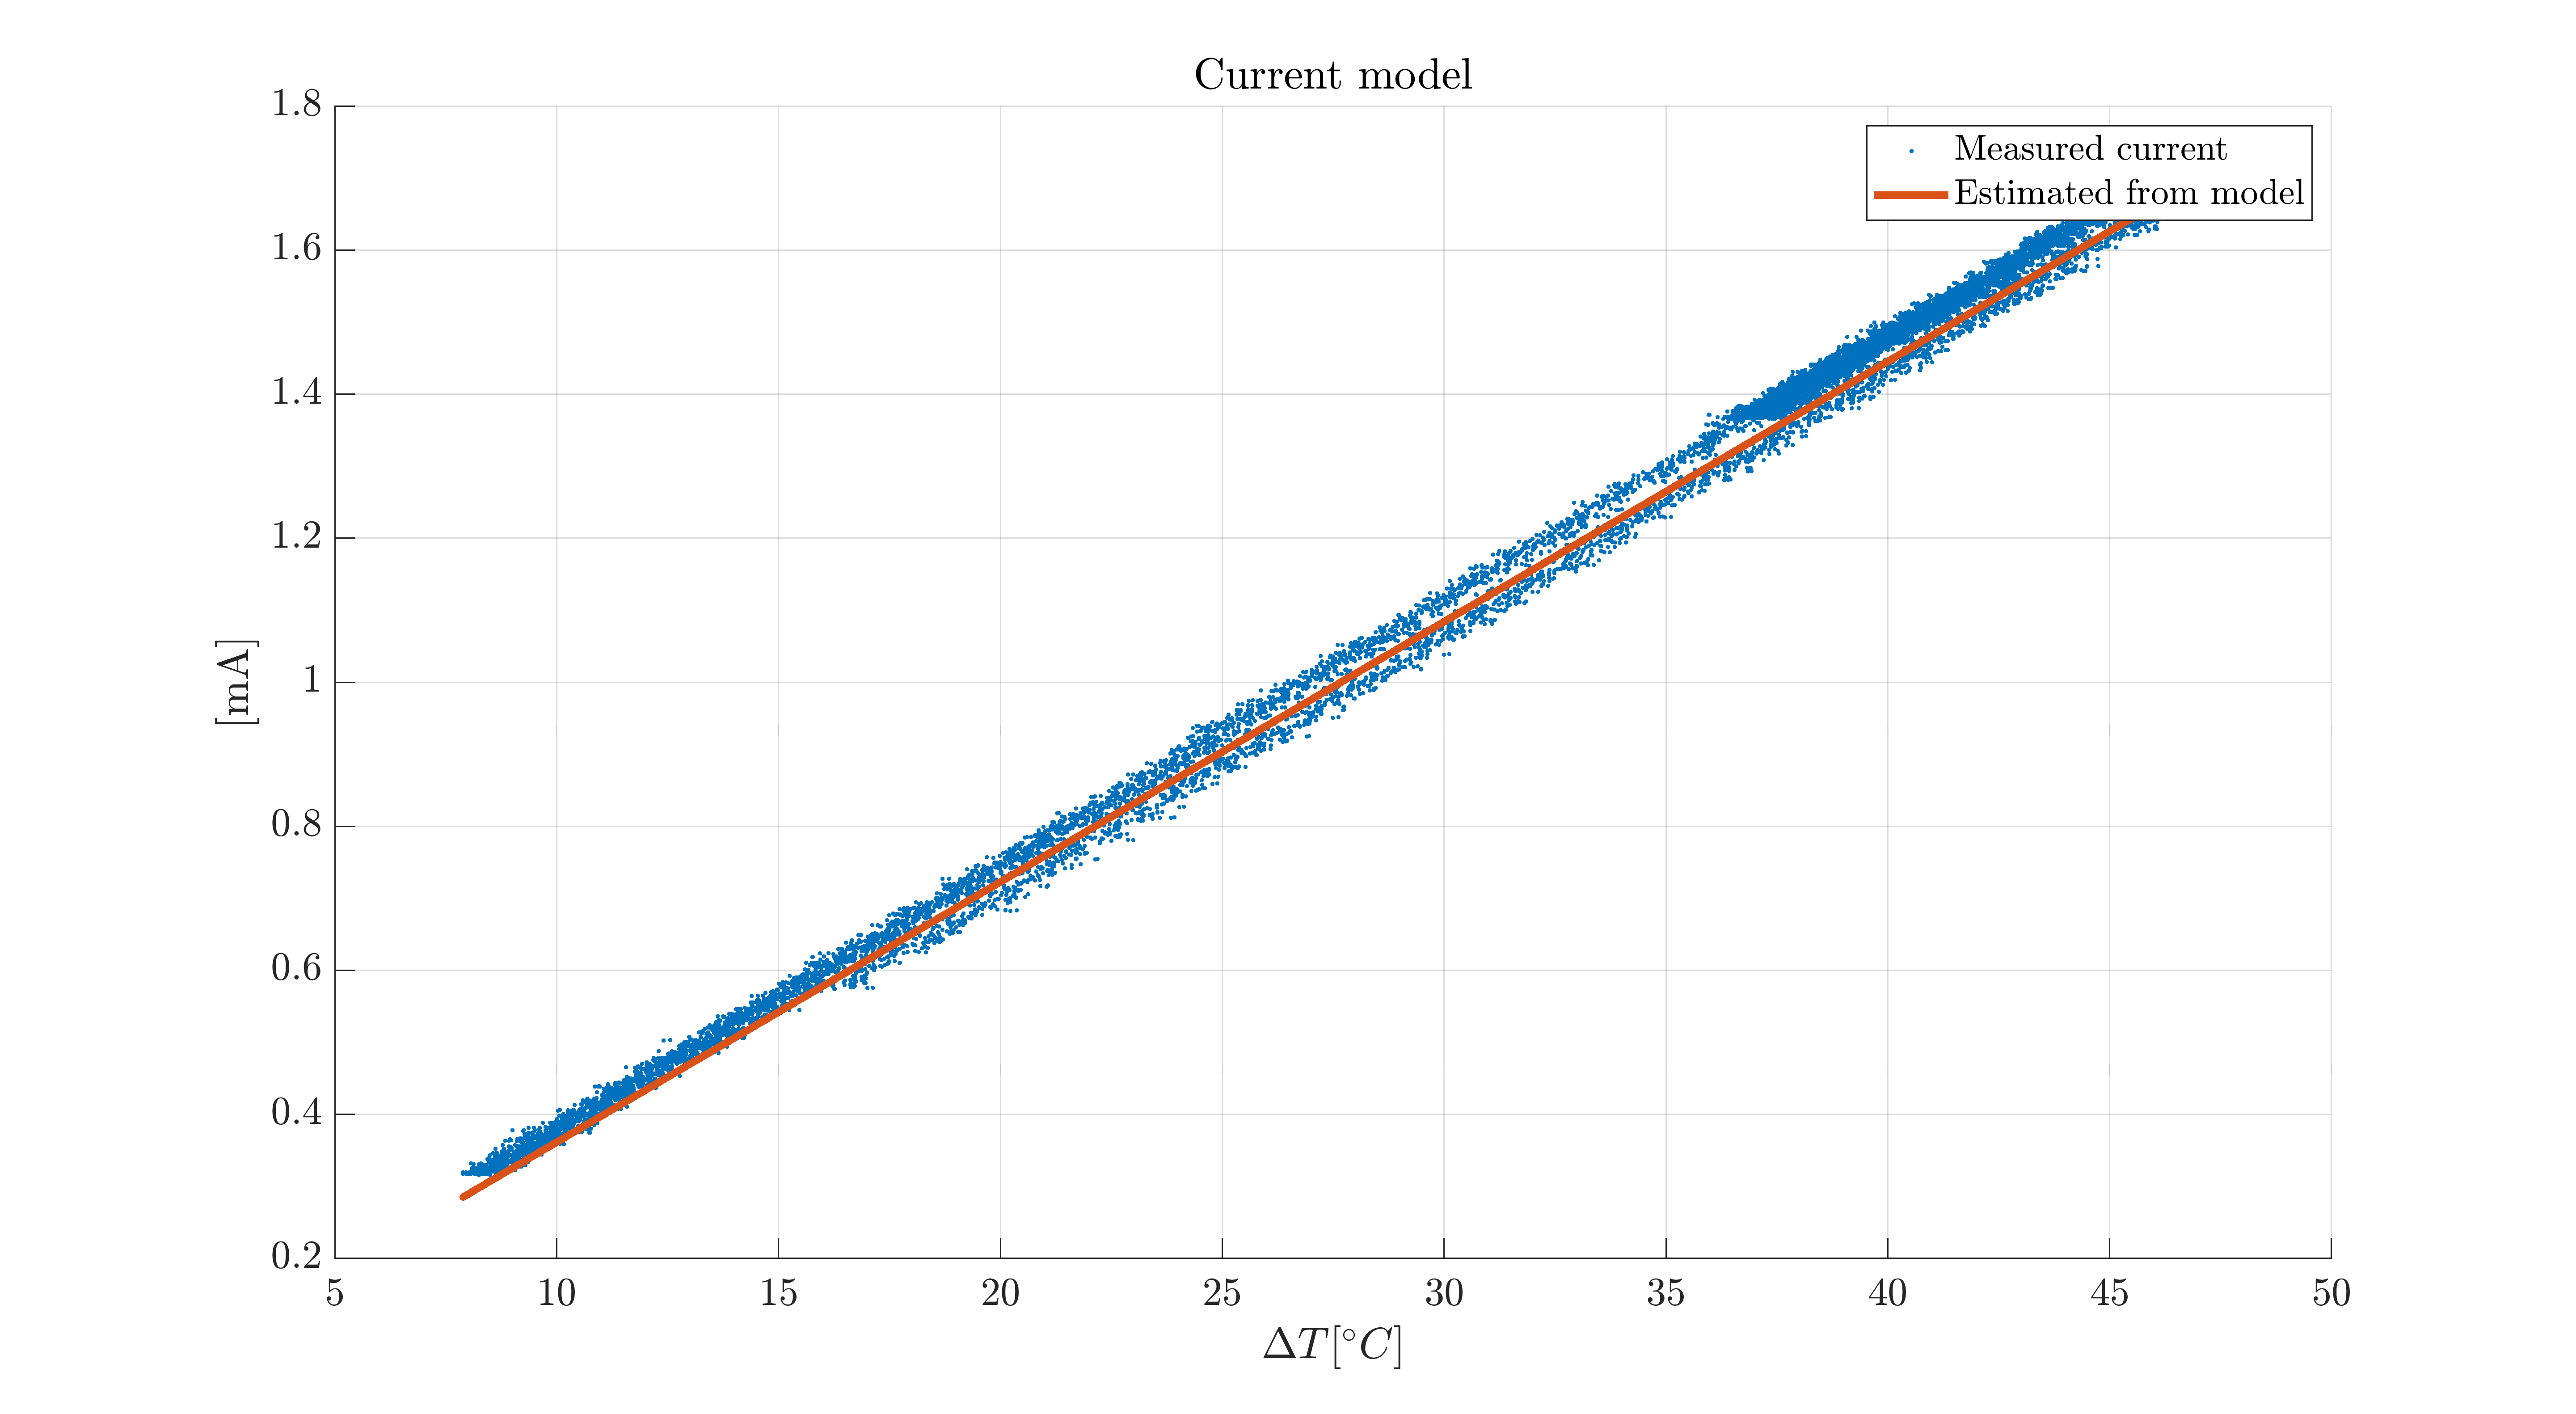
\includegraphics[width=0.45\textwidth]{assets/Current model.png}
    \caption{Measured current vs model estimate.}
    \label{fig:voc_current_model}
\end{figure}
